% Set document type
\documentclass[conference]{IEEEtran}

% Packages
\usepackage{graphicx}
\usepackage{flushend}
\usepackage{cite}

% For highlighting areas to change, use the color package
\usepackage{color}

% Fix hyphenation
\hyphenation{op-tical net-works semi-conduc-tor}

% Start of document
\begin{document}
\bibliographystyle{plain}

% Title and author block
\title{Stencil Code Optimization for GPUs Through Machine Learning}
\author{\IEEEauthorblockN{Adam Barker}
\IEEEauthorblockA{%College of Engineering and Applied Science\\
University of Colorado at Colorado Springs\\
abarker2@uccs.edu}}
\maketitle

% Abstract
\begin{abstract}
	The microprocessor field today has begun to reach its limits as power and thermal constraints have been met and no longer can much leverage of increasing the processor's clock speed be achieved. Thus, much of the scientific and engineering community has shifted to using many-core architectures, such as GPUs, in order to do highly-parallel computations. However, the switch to GPU has created problems of its own as developers of GPU kernels must understand the low-level specifications of the hardware in order to properly optimize code. This paper will focus on the use of genetic algorithms to guide the optimization of stencil codes on NVIDIA's Compute Unified Device Architecture (CUDA) based GPUs and GPGPUs.
\end{abstract}

% Introduction
\section{Introduction}
	Due to power and thermal constraints, the domain of micro-processors no longer benefits from increases in clock frequency\cite{Datta}. This problem has shifted the focus of parallel computing to advanced many-core architectures, such as those present among GPUs. However, this transition has led to problems in software development as programmers have difficulty in successfully optimizing GPU kernels to efficiently use the resources provided by the architecture. This hampering occurs regardless of new programming models such as CUDA and OpenCL as programmers have difficulty understanding the underlying architecture, which is necessary to correctly optimize kernels for the GPU\cite{Zhang}. Also, NVIDIA typically updates its GPU architecture every one to two years, each with brand new layouts which make programmers have to learn the new architecture in order to optimize code correctly. Stencil computations are widely used in scientific computing on structured grids and in Partial Differential Equation (PDE) solvers for domains such as computational fluid dynamics and other finite-difference computations\cite{Mici, Nguy, Jaeger, Datta, Gana, Zhang, NVIDIA}.

	Stencil computations use nearest-neighbor calculations to approximate the value of the current node. In explicitly iterative stencil computations, a computationally-intensive kernel is used to update all nodes in the grid at distinct time steps. Due to this, stencils benefit highly when placed on SIMT (Single Instruction Multiple Thread) architectures, such as those on GPUs. However, due to the massive number of threads being run on a single grid, the number of memory accesses for each time step is enormous and thus, stencil computations are generally memory-bound. These memory accesses typically contain overlap between threads as each node shares neighbors with other nodes, so exploiting this property allows for optimizations that are crucial to leveraging data-level parallelism inherent in these computations\cite{Zhang}.

%\begin{figure}[h]
%	\centering
%		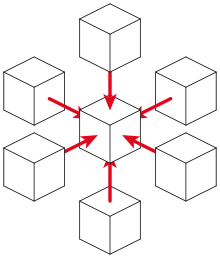
\includegraphics[width=5cm]{stencil-7.png}
%		\caption{A 6-point Von-Neuman stencil (credit: wikipedia.org)}
%\end{figure}

	Auto-tuning of stencil kernels is an active field of study that aims to work around the necessity of developer knowledge of the low-level specifications of the architecture in order to optimize the kernel. However, these auto-tuners may have to look in a parameter space that is upwards of 40 million unique combinations that may take months to fully check every single one for optimal performance\cite{Datta}. Therefore, machine learning should be a valid option for automatic optimization as it is capable of searching through large parameter spaces quickly by making predictions about the parameter space in order to find a near-optimal configuration. Using machine learning can also overcome another downfall of auto-tuning in that each auto-tuner must be run every time for every stencil code and machine, whereas a machine learning algorithm can make predictions based on previous results, greatly improving run time.

	This work focuses on optimizing stencil codes on CUDA-enabled NVIDIA GPUs. The list of GPUs used to conduct this research consists of two consumer-level GPUs (GTX 680, GTX 480) and one General-Purpose computing GPU (Tesla C2050). Between the chips, two architectures are tested: the GTX 480 and the Tesla C2050 use the Fermi architecture, whereas the GTX 680 uses the latest Kepler architecture. It should be noted that the Tesla C2050 is a GPGPU that is capable of performing double-precision floating point operations, whereas the GTX 480 and GTX 680 can only achive 1/8 the performance for double-precision as they lack the specialized hardware that is on the Tesla GPU\cite{NVIDIA}. 

% Related Work
\section{Related Work}
	Due to the high-memory bandwidth requirements needed for stencil computations, much of the research done for optimization focuses primarily on memory layout techniques and exploiting lower levels of memory such as cache and shared memory. One technique is 2.5D blocking in order to create the grid layout in memory by only finding the x and y values of the thread block and keeping the z axis constant\cite{Datta}. However, another paper has been written on a different blocking scheme that is optimal for stencil computations called 3.5D blocking which combines 3D blocking with 2.5D blocking in order to lower the amount of memory accesses for a stencil code\cite{Nguy}. Another promising research paper was done on efficient data layout for stencil codes on GPUs and similar multithreaded architectures which provides another key optimization to incorporate in this research\cite{Jaeger}. 

	{\color{red}Recent work in machine learning applications for guiding stencil code optimization, a case study was employed to see if statistical machine learning and genetic algorithms could be used to guide the optimization of stencil kernels on multicore architectures\cite{Gana}.}

	Also, many auto-tuning and auto-generation techniques have been explored, most notably research done on the auto-tuning of 3D stencil codes on GPU clusters, which details a rigorous auto-tuning and auto-generation framework for CUDA devices, which can be incorporated into our work by benchmarking our machine learning algorithm's speed against the speed of a similar auto-tuning mechanism based on the research\cite{Zhang}. 

% Motivation
%\section{Motivation}
%	Due to the large number of optimizations to be considered and difficult architecture layouts to master, machine learning is a desirable approach to automatically determining optimized stencil kernel configurations quickly on any architecture. 

% Conclusion
%\section{Conclusion}
%	Ultimately, this project aims to create a machine learning algorithm based on statistical machine learning and genetic programming in order to create a fast, efficient alternative to the auto-tuners and hand-optimizations currently done for stencil computations on GPUs. Although this research will focus only on using these techniques to optimize CUDA GPUs, it will hopefully be able to be applied to other architectures as well, as one implementation was already done for multicore CPU architectures\cite{Datta}. Also, this research is done in the hopes that it will create a movement toward more research projects to be done in the field of GPU stencil code optimizations, as these computations are so widely used in the industry today.

% Acknowledgements
\section{Acknowledgements}
	This research is supported by NSF REU Grant 1359275

{ \vspace*{\columnsep} }

\bibliography{myBib}

% That's all folks
\end{document}
